\documentclass[12pt]{article}
\usepackage[margin=1in]{geometry}
\usepackage{enumitem}
\usepackage{caption}
\usepackage[subrefformat=parens,labelformat=parens]{subcaption}
\usepackage{graphicx}
\usepackage{cite}
\graphicspath{{figures/}}

\title{
  \vspace{-2cm}
  CSE 455 Homework 5 \\
  \author{Yoshihiro Kumazawa}
}

\begin{document}
\maketitle

\section{Installing PyTorch}
Done!

\section{Find the best network}
\subsection{Training a classifier using only one fully connected Layer}
See Figure~\ref{fig:2_1}. We can say that the the model successfully trained since the loss is decreasing throughout the training process and there is a healthy gap between the training accuracy and testing accuracy.

\subsection{Training a classifier using multiple fully connected Layers}
See Figure~\ref{fig:2_2}. The training is not successful because the testing accuracy plateaus whereas the training keeps increasing.

\subsubsection{Question}
See Figure~\ref{fig:2_2_1}. The model accuracy is significantly worse than the previous model. This is because the model is expressively limited since it has less non-linearity. The model can actually become just as good as LazyNet since without activations, the forward pass is just a couple of matrix multiplications, which is nothing but a single matrix multiplication by the composed matrices. But somehow, by separating the weight update process in back propagation, it achieves a slightly higher accuracy than LazyNet.

\subsection{Training a classifier using convolutions}
Our CoolNet is based on LeNet~\cite{Lecun98gradient-basedlearning}. In addition, batch normalization~\cite{pmlr-v37-ioffe15} is performed after each convolutional layer and linear layer except the final layer in order to get the network to converge faster. As a result, the network got higher accuracy then the previous models. See Figure~\ref{fig:2_3_bs4} for the training result.

\subsubsection{Question}
We tried batch sizes of 4, 32 and 256. See Figure~\ref{fig:2_3_bs4}, Figure~\ref{fig:2_3_bs32}, and Figure~\ref{fig:2_3_bs256} respectively. The loss curves account for the difference. Batch size 4 is so small to compute gradients accurately that the loss does not decrease sufficiently. On the other hand, when the batch size is 256, the total iteration number is much smaller and the training loss did not saturate. Among these 3 models, the model trained with batch size 32 performed best.
\begin{figure}
  \begin{subfigure}{0.16\textwidth}
    \centering
    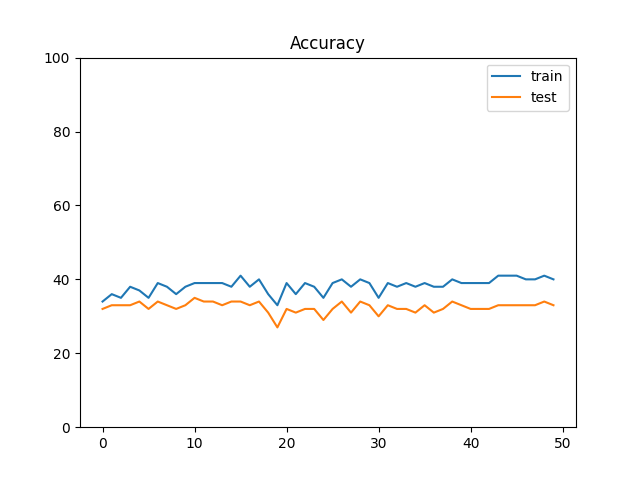
\includegraphics[width=\linewidth]{accuracies_2_1.png}
  \end{subfigure}
  \begin{subfigure}{0.16\textwidth}
    \centering
    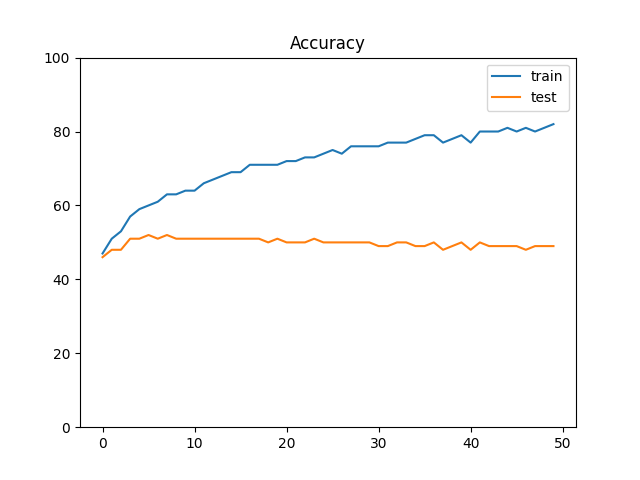
\includegraphics[width=\linewidth]{accuracies_2_2.png}
  \end{subfigure}
  \begin{subfigure}{0.16\textwidth}
    \centering
    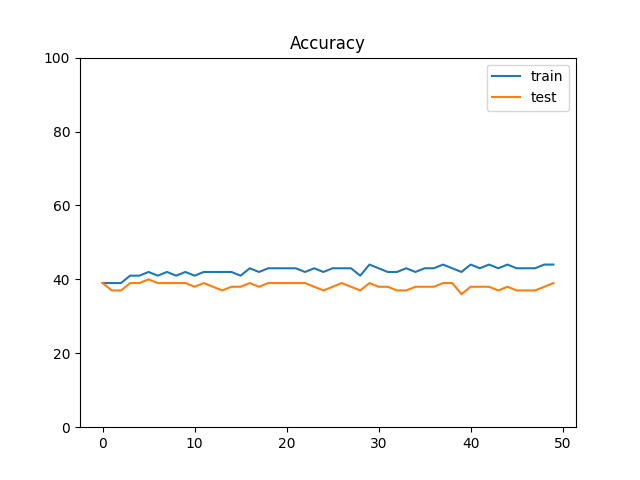
\includegraphics[width=\linewidth]{accuracies_2_2_1.png}
  \end{subfigure}
  \begin{subfigure}{0.16\textwidth}
    \centering
    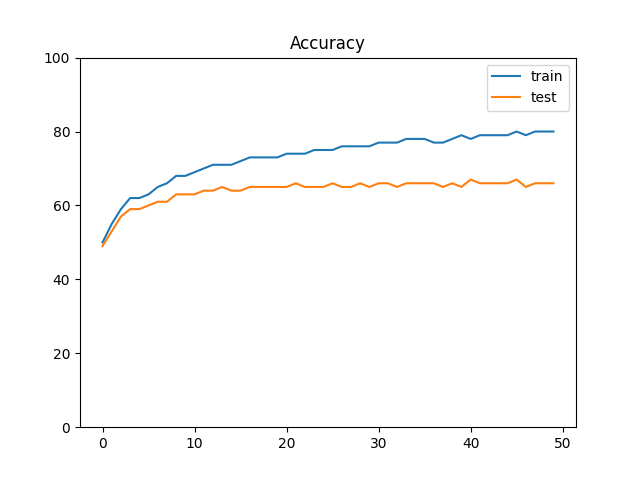
\includegraphics[width=\linewidth]{accuracies_2_3_bs4.png}
  \end{subfigure}
  \begin{subfigure}{0.16\textwidth}
    \centering
    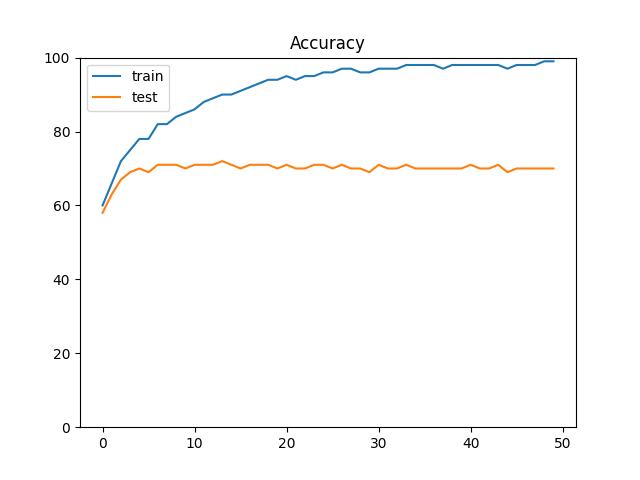
\includegraphics[width=\linewidth]{accuracies_2_3_bs32.png}
  \end{subfigure}
  \begin{subfigure}{0.16\textwidth}
    \centering
    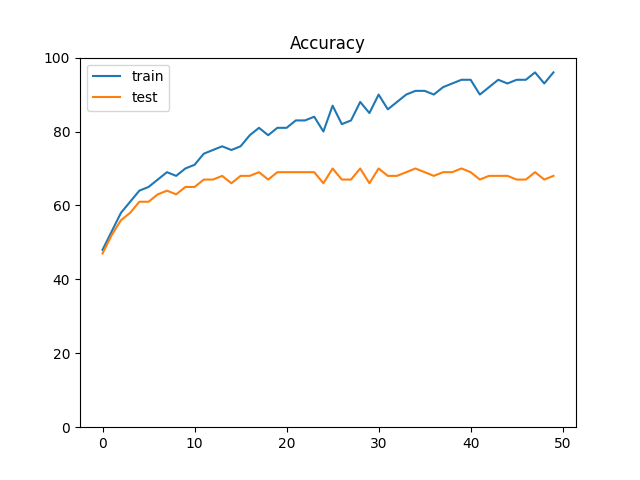
\includegraphics[width=\linewidth]{accuracies_2_3_bs256.png}
  \end{subfigure}

  \begin{subfigure}{0.16\textwidth}
    \centering
    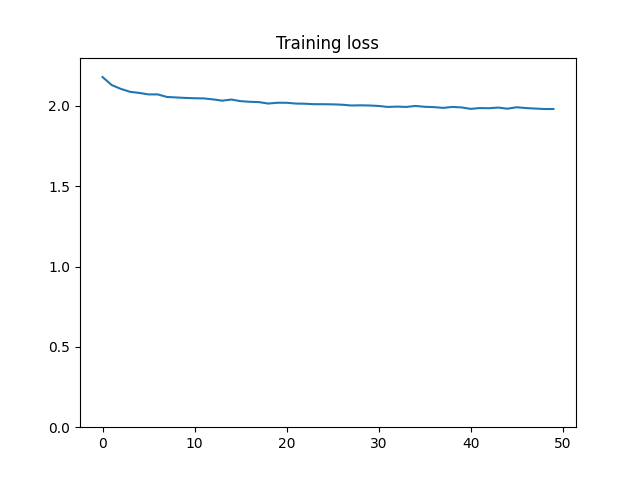
\includegraphics[width=\linewidth]{loss_2_1.png}
    \caption{}
    \label{fig:2_1}
  \end{subfigure}
  \begin{subfigure}{0.16\textwidth}
    \centering
    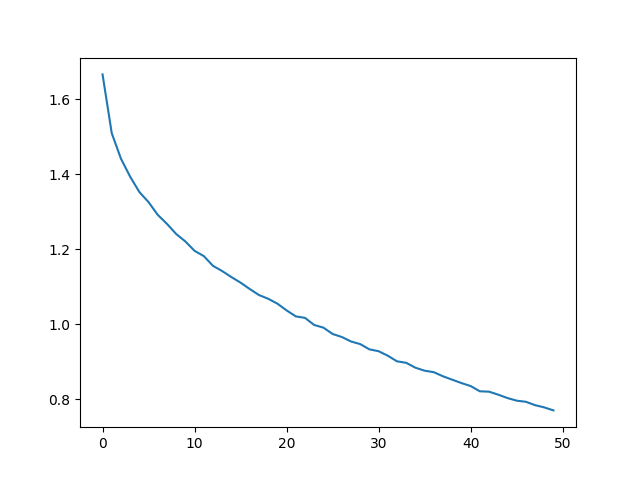
\includegraphics[width=\linewidth]{loss_2_2.png}
    \caption{}
    \label{fig:2_2}
  \end{subfigure}
  \begin{subfigure}{0.16\textwidth}
    \centering
    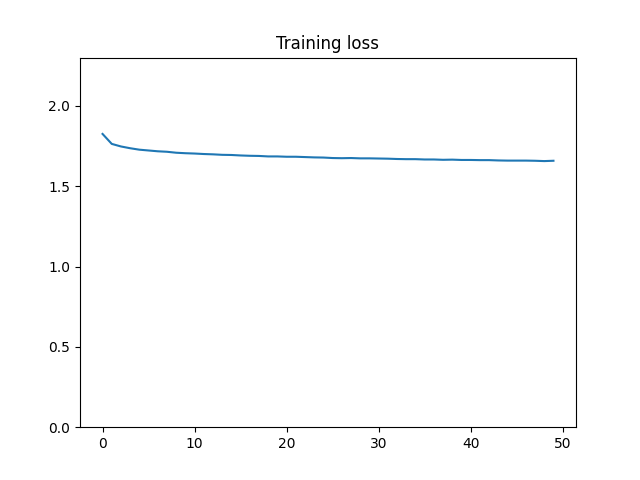
\includegraphics[width=\linewidth]{loss_2_2_1.png}
    \caption{}
    \label{fig:2_2_1}
  \end{subfigure}
  \begin{subfigure}{0.16\textwidth}
    \centering
    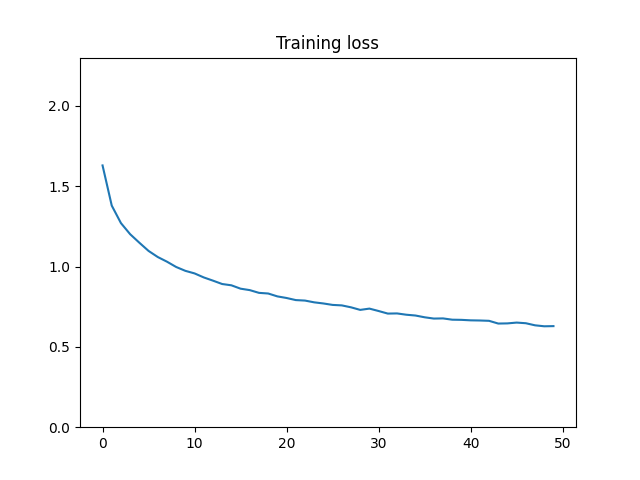
\includegraphics[width=\linewidth]{loss_2_3_bs4.png}
    \caption{}
    \label{fig:2_3_bs4}
  \end{subfigure}
  \begin{subfigure}{0.16\textwidth}
    \centering
    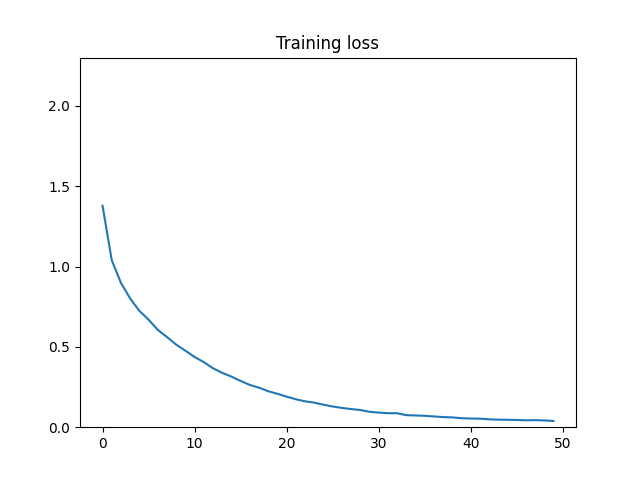
\includegraphics[width=\linewidth]{loss_2_3_bs32.png}
    \caption{}
    \label{fig:2_3_bs32}
  \end{subfigure}
  \begin{subfigure}{0.16\textwidth}
    \centering
    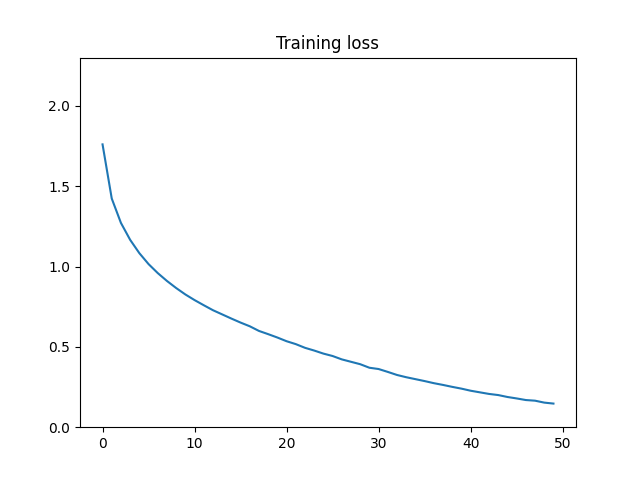
\includegraphics[width=\linewidth]{loss_2_3_bs256.png}
    \caption{}
    \label{fig:2_3_bs256}
  \end{subfigure}
  \caption{Training results of LazyNet, BoringNet and CoolNet: \subref{fig:2_1} LazyNet, \subref{fig:2_2} BoringNet, \subref{fig:2_2_1} BoringNet without activations, \subref{fig:2_3_bs4} CoolNet with batch size 4, \subref{fig:2_3_bs32} CoolNet with batch size 32, \subref{fig:2_3_bs256} CoolNet with batch size 256.}
  \label{fig:images}
\end{figure}

\section{How does learning rate work?}

\section{Data Augmentation}

\section{Change the loss function}

\bibliography{report}
\bibliographystyle{plain}
\end{document}
